
\chapter{Twizzler: An Implementation}\label{ch:twizzler}

\section{Objects}

\unedit{
    The kernel provides services for object management, such as creating and deleting objects.
    Objects are created by the \texttt{create} system call, which
    returns an object ID\@. A program may also optionally provide an existing object ID to the
    \texttt{create} call, stating that the new object should be a copy of the existing one, for which
    \Twizzler uses copy-on-write. The new ID is a number that
    is unlikely to collide with existing IDs in the 128~bit ID space, and can be assigned using a technique
    that supports this requirement (random, hashing, \emph{etc}.).
    Some forms of ID assignment support a form of access
    control: a program can only access an object whose ID it knows. \Twizzler provides
    object naming as well, discussed in Section~\ref{sec:invariant_pointers}.

    Objects may be be deleted via the \texttt{delete} system call.
    %, however deletion is not immediate.
    Like \unix's \texttt{unlink}, objects are reference counted, where a reference refers to a mapping
    in an address space. Once the reference count reaches zero, the object may be deleted. During
    deletion, an object may be optionally marked as ``hidden'', causing new mapping requests for this
    object to fail.
}

\subsection{Creation}

\subsection{Deletion}

\section{Dealing with Ephemera}

\subsection{Threads}

\unedit{\Twizzler provides a set of threading primitives for applications. Threads in \Twizzler are always
    attached to a view and one or more security contexts. Threads may communicate with each other using
    shared memory and can signal each other with a system call.
    Since everything in \Twizzler is an object, each thread has a state object associated
    with it. Signals can be raised assuming the raiser has appropriate permissions on the state object,
    and the state object contains information about the thread.

    A key primitive in \Twizzler is the \texttt{thread-sync} system call. This call operates similar to
    \texttt{futex(2)} on Linux, except that it supports waiting on and waking up a number of different
    words of memory simultaneously. Multi-word thread-sync is necessary to support
    \texttt{select(2)}-like or \texttt{poll(2)}-like operations in a system where all data access is
    done with memory semantics. \Twizzler's standard library exposes an API for event handling that uses
    multi-world thread-sync, where objects may expose a set of ``events'' that can be triggered and waited for. This is
    used in numerous places to implement event handling for multiple communications streams implemented
    in objects.
}

\subsection{Program Instancing}


\unedit{
    \subsubsection{Ephemeral State Management with Views}
    \label{sec:view}
    \iffalse
        \dab{What we could do here is reframe this section and rename it. Sure, virtual addresses are needed, and it's how
            we map things. But there's a much more fundamental thing that we are doing here. We're providing a
            mechanism to mesh together ephemeral "moments of computation" (threads) with persistent data. We can
            add a figure here that's \texttt{threads (computation)---views (ephemeral state
                mapping)---persistent data} or something. The question is, is this something that we would want to
            include in a future publication?}
    \fi

    Despite \Twizzler's focus on persistent data, many components of our hardware and applications are
    built around ephemeral constructs. For example, threads are ephemeral ``moments of computation''
    that act on persistent data, while the programs that they execute often expect some ephemeral
    private data (\eg the data segment and the stack). While virtual addresses are the wrong abstraction
    for persistent data access, modern hardware provides (and often requires) the use of virtual address
    hardware that we can leverage for protection and isolation, adding additional ephemeral state.

    \Twizzler defines objects called ``views'', which coalesce the state
    and context necessary to support ephemeral constructs like threads and application instances into
    \Twizzler objects. A significant part of that state is ephemeral virtual address mappings; \Twizzler
    provides access to persistent objects by mapping them into the virtual address space
    behind-the-scenes (via \libcore). The view object contains structures to define the layout of the
    virtual address space which the kernel reads and uses to program the MMU accordingly. Figure~\ref{fig:view2} shows how
    views ``mesh'' ephemeral threads with persistent data by providing them a context to operate in.
    Since view objects are normal \Twizzler objects, they can be persisted, allowing
    us to recover application state after power cycles.

    \begin{SCfigure}
        \centering
        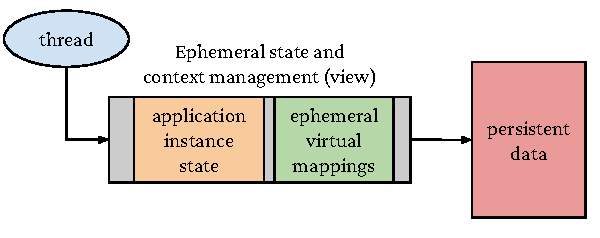
\includegraphics[width=\linewidth]{fig/view2}
        \caption{View objects in \Twizzler. Views manage ephemeral constructs and state, giving threads
            the necessary context to execute and access persistent data.}
        \label{fig:view2}
    \end{SCfigure}


    By coalescing this ephemeral state
    into an object, we make it possible for applications to manage it directly with minimal kernel
    involvement. Avoiding the kernel is natural---all data access already does this in \Twizzler, so
    adding a separate kernel API to manage this state would add complexity---and reduces the number of
    system calls needed when mapping objects. Additionally, avoiding the kernel necessitates an
    increased address space management responsibility for userspace. For example, executable loading
    and mapping is largely handled without the kernel.



    \iffalse
        Although virtual addresses are the wrong abstraction to use for persistent
        data access, we do leverage virtual address hardware in modern processors for isolation and
        protection.
        \Twizzler provides access to persistent objects by mapping
        them into the virtual address space behind-the-scenes (via \libcore).
        %; applications need not operate on this level of abstraction directly).
        This generates many mapping operations to access persistent data, so requiring system calls would be
        costly. Additionally, our kernel avoidance necessitates an increased address space management
        responsibility for userspace. For example, executable loading and mapping is handled largely
        without the kernel.
        %, and modern software frameworks may
        %map data into address spaces frequently~\cite{2016posix}. Requiring system calls would
        %be costly, especially when we are trying to avoid kernel boundary crossings.

        To support userspace manipulation of address spaces,
        the kernel and userspace share an object (called a ``view'') that
        defines an address space layout. The view is just a normal
        object, and so standard access control mechanisms apply to enforce isolation.
        When applications map objects into their address space, they update the view to specify
        that a particular object should be addressable at a specific location.
        The kernel then reads the object and determines the
        requested layout of the virtual address space. The view object is laid out like a page-table (shown
        in Figure~\ref{fig:view}), where
        each entry in the table corresponds to a slot in the virtual address space.
        Each table entry contains an object ID and read, write, and execute protection bits to further
        protect object access (like \texttt{PROT\_*} in \texttt{mmap}).
    \fi

    Figure~\ref{fig:view} shows how view objects lay out the address space of any threads running inside
    that particular view. View objects are manipulated by userspace and interpreted by the kernel. When
    applications map objects, they update the view to specify that that object should be addressable at
    a specific location. On a page-fault, the kernel reads the view and maps the object at the requested
    location. The view object is laid out like a page-table, where each entry in the table corresponds
    to a slot in the virtual address space. Each table entry contains an object ID and requested
    protection bits to further protect objects atop access control mechanisms (similar to
    \texttt{PROT\_*} in \texttt{mmap}).

    \begin{SCfigure}
        \centering
        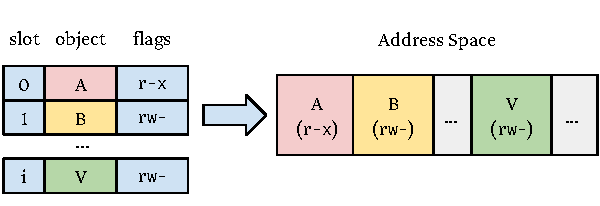
\includegraphics[width=\linewidth]{fig/view}
        \caption{Layout of a view object. The kernel consults the view object's mapping on page-fault,
            and maps in the requested objects at the appropriate location in the virtual address space.}
        \label{fig:view}
    \end{SCfigure}

    %When a fault occurs, the kernel checks if the faulting thread is a \Twizzler thread, and if so,
    %diverts it to a different fault handler.  The new
    When a page-fault occurs, the fault handler tries to handle the fault by either doing copy-on-write,
    checking permissions, or by trying to map an object into a slot if the view object requested one.
    If it cannot handle the fault (due to a protection error or an empty entry in the view
    object), it elevates the fault to userspace where \libcore handles it, possibly by killing the
    thread, or possibly by mapping an object if the slot is ``on-demand''. This is similar to userspace
    paging systems~\cite{l4,accetta:usenix86s}. When the kernel
    maps an object into a slot, it updates the address space's page-tables appropriately.

    Applications can add objects to a view with the \texttt{view\_set} function. The caller specifies a
    target object and a set of protections (see \S~\ref{sec:invariant_pointers}), and a slot in which to
    map the object. However, applications rarely invoke this function directly---instead,
    \texttt{libtwz} provides a higher-level API to allow applications to operate above the level of
    manually mapping objects. The standard library also provides access to other utility functions for
    views (such as querying state, creating new views, and copying views). These functions, by default,
    operate on a thread's current view, but they may also optionally operate on any other view object,
    which allows \Twizzler to implement operations with semantics similar to \texttt{fork} and \texttt{execve}.

    When threads add entries to a view object they need not inform the kernel---when
    a fault occurs, the kernel will read the entry as needed. However, when \emph{changing} or
    \emph{deleting} an entry, threads must inform the kernel so it can update existing page table entries.
    We provide two system calls for views. The \texttt{become} system call allows a thread to
    change to a new view, which might be used to execute a new program or jump across programs to, for
    example, accomplish a protected task. \Twizzler's access control system prevents this from happening
    arbitrarily. The second system call is \texttt{invalidate\_view}, which lets a thread inform the
    kernel of changed or deleted entries.

    View objects not only reduce kernel boundary crossings, but they also improve the resumability of
    the system. After a power cycle, the OS now has information on which objects were mapped and where,
    improving the ability of threads to pick up where they left off. Additionally, view objects
    facilitate the sharing of address spaces between threads, since they can both synchronize on
    modifying a given view object and need not duplicate information. Note that the particular contents
    of a view object are system-specific. On virtual memory systems, one of their jobs is to manage
    ephemeral virtual mappings, while on other architectures their jobs may be to manage, \eg, segment
    tables. However, in all cases, views provide a mechanism for managing ephemeral state while
    providing enough context for threads to execute.
}



\unedit{
    \paragraph{Pointer Translation.}

    Current processors provide only a virtual memory abstraction, so applications must do some
    extra work to dereference a pointer, \emph{translating} a pointer from its persistent form into a
    virtual address. This does not affect the
    \emph{stored} pointer, which is still persistent and independent of any translation or address
    space. Thus multiple applications, possibly with different address space layouts, can translate the
    same pointer at the same time without coordination.

    Pointer translation occurs with the help of two \libcore functions: \texttt{ptr\_lea}
    (load effective address) and \texttt{ptr\_store}. When a program dereferences a pointer, it first
    calls \texttt{ptr\_lea}. The pointer is resolved into an
    object-ID and offset pair through a lookup in the FOT, after which \libcore determines if the
    referenced object is already mapped (by maintaining per-view metadata). If not, it picks an empty
    slot in the view and maps the object there (a cheap operation that does not invoke the kernel). Once mapped,
    \libcore combines the object's temporary virtual base address with the offset, and
    returns the new pointer. The \texttt{ptr\_store} function does the opposite of
    \texttt{ptr\_lea}---it turns a virtual pointer into a persistent one. While these are done manually
    in our implementation, we plan to implement compiler support to emit these calls automatically.


    FOT management is handled by \libcore.
    While a lookup in the FOT is a simple array-indexing operation, a
    store may require adding to the FOT\@. To avoid duplicate entries, \libcore walks
    the FOT looking for a compatible entry.
    If one is not found, it atomically reserves a new entry and fills it (flushing cache-lines to
    persist it) before storing the pointer. The \texttt{ptr\_store} operation is less
    common than \texttt{ptr\_load}, and in the future we may include additional caching
    metadata that would speed-up the FOT walk (such as storing recent IDs).


    Translating pointers has a small overhead
    (\S~\ref{sec:res}) and the result can be cached. \Twizzler
    improves performance via a per-object cache of prior translations.
    %to speed up external
    %references.
    The common case, intra-object pointers, does not require an external
    lookup and is implemented as a simple bitwise-or operation.
    \iffalse
        \paragraph{Persistent and Volatile Pointers}
        \dab{THIS IS ALL NEW}

        Note that \Twizzler does not attempt to limit the creation of pointers between volatile and
        persistent data. This is an example of ongoing \NVM research that \Twizzler does not want to
        prematurely limit. However, we expect that this is the right decision regardless, as the goal of the
        OS is to provide a framework for higher-level abstraction, not to prescribe limitations that could
        be better handled at the language level. For example, there is a wealth of ongoing research in
        language support for \NVM \dab{CITE}, and one particularly important aspect is typing volatile and
        persistent pointers. We believe that this should be handled as a language feature with sufficient OS
        support, so we are leaving ourselves open to future research.

        Similar to the discussion of object lifetime in \S~\ref{sec:obj}, its pointers from a persistent
        object to a volatile object that can cause problems. Internal (intra-object) pointers are not a
        problem, since they have the same lifetime as the data that they point to. Thus, since it's only
        external, inter-object pointers that can be an issue here, we are leaving open the possibility that
        a language with \Twizzler support could use FOT data to encode type or lifetime information for
        pointers. One angle of future work we would like to explore is modifying a language to natively
        support this idea. For example, Rust already has explicit semantics for data lifetime and
        infrastructure for enforcing ``safer'' memory references.
    \fi
}
\section{Security}

\section{\textsc{unix} Compatibility}

\unedit{
    \subsection{Porting Additional Applications}
    In general, porting in \Twizzler is straight-forward. We have a collection of tools that provide a
    framework for compiling software using the \Twizzler toolchain against other ported software and
    libraries. Since we have chosen \texttt{musl} as our standard C library, many applications work
    already with minor changes. However, it is often the case that applications require
    some small tweaks to get running---for example, configuration paths---an experience common for anyone who has ported software to a new
    operating system.

    To date, we have ported a number of tools one would expect to find on a \unix system, such as
    \texttt{busybox} (providing numerous command-line utilities), \texttt{bash}, \texttt{vim},
    \texttt{gcc}, \texttt{binutils}, and others. Many of these programs required little or no
    modification. Of course, this means that they do not gain some of the benefits \Twizzler's model
    provides, since they still operate on persistent data with a POSIX model, however our goal in
    porting these tools was not to improve their performance, it was to provide a somewhat familiar
    environment for users.

    Of course, perfect emulation of a Linux kernel is a huge effort, and it is not the primary goal of
    our research. As a result, not all system calls are implemented and Linux features like
    \texttt{procfs} are lacking. This means that some programs may require features that are not yet
    implemented, and therefore require modifications to \texttt{twix} to run. However, as we continue to
    port software, \texttt{twix}'s coverage of Linux features grows, making future porting easier. We
    will continue to implement more support in \texttt{twix} for applications as needs arise. Note that
    many applications (even complex applications like \texttt{gcc}) often boil down to reading and
    writing files and managing processes, all of which is implemented.
}

\unedit{
    \subsection{Twix System Call Overhead}

    Our \unix emulation layer, \texttt{twix}, is meant to provide compatibility for legacy applications.
    While we expect that applications will wish to take full advantage of \NVM and \Twizzler's
    improvements in programmability and performance, we can still provide a small benefit
    for applications that rely on \texttt{twix} to provide POSIX-like I/O. Access to \texttt{twix} is
    done by \texttt{musl}, the C library we use, when it would normally perform a system call to a Linux
    kernel. We replaced all instances of the \texttt{syscall} instruction in C and assembly code in
    \texttt{musl} with a \texttt{call} instruction to an entry point in \texttt{twix}. This entry point,
    despite being a function call, obeys the Linux system call ABI (\eg which registers hold
    parameters). Thus while it has significantly less overhead than a full system call and context
    switch, it does still have higher overhead than a normal function call since it must back up and
    restore all registers.


    \begin{SCtable}[b]
        \centering
        \caption{Latency of selected \texttt{twix} system calls compared to Linux system calls.}
        \begin{minipage}{\linewidth}
            \centering
            \begin{tabular}{c | c | S[table-format=6.1]@{\,\,\( \pm \)\hspace{-7mm}} S[table-format=0.1]}
                \textbf{System Call} & \textbf{OS} & \multicolumn{2}{c}{\textbf{Average Latency (ns)}}       \\
                \hline
                \hline
                \texttt{getpid}      & Linux       & 98.7                                              & 2.3 \\
                                     & Twizzler    & 10.2                                              & 0.2 \\
                \hline
                \texttt{read}        & Linux       & 321.4                                             & 0.2 \\
                                     & Twizzler    & 55.4                                              & 0.2 \\
            \end{tabular}
        \end{minipage}
        \label{tbl:twix}
    \end{SCtable}

    Table~\ref{tbl:twix} shows the latency of some selected system calls on both Linux and \Twizzler
    (implemented via \texttt{twix}). As expected, \texttt{getpid}'s overhead is small on both systems,
    but on \Twizzler it is significantly lower. The difference, in this case, comes largely from the
    kernel entry overhead. A small amount of additional overhead comes from
    \texttt{twix} matching the Linux system call ABI and having to call its \texttt{getpid}
    implementation through a lookup table.

    We also measured the latency of a call to \texttt{read} for a file. We chose to do reads on cached
    files for a small number of (already cached) bytes to avoid device transfer overhead. Performing a file read on
    \Twizzler often amounts to a call to \texttt{memcpy}, so applications that perform large numbers of
    small reads could see some benefit. In contrast, on Linux, the kernel needs to traverse internal
    file structures, the page-cache, and possibly file system structures.
    However, as we said, \texttt{twix} is intended for legacy
    support, not performance improvement despite the lower system call overhead.
    %As \texttt{read}
    %lengths increase, we expect to see the system call overhead diminish relative to the cost of copying
    %bytes into the buffer.
}

\section{Access to Legacy Devices}

\subsection{Drivers}

\subsection{Block Storage}